\documentclass[11pt,a4paper]{article}
\usepackage{booktabs}
\usepackage{longtable}
\usepackage{array}
\usepackage{amsmath}
\usepackage{graphicx}
% Manual page layout (geometry.sty is not installed in this MiKTeX tree)
\setlength{\textwidth}{16.8cm}
\setlength{\textheight}{23.8cm}
\setlength{\oddsidemargin}{-0.44cm}
\setlength{\evensidemargin}{-0.44cm}
\setlength{\topmargin}{-0.7cm}
\setlength{\headheight}{0pt}
\setlength{\headsep}{0.3cm}
\setlength{\footskip}{0.8cm}
\setlength{\belowcaptionskip}{7pt}
\setlength{\itemsep}{2pt}
\setlength{\topsep}{2pt}
\setlength{\leftmargini}{1.5em}
\pagestyle{plain}

\begin{document}

\begin{center}
{\Large\bfseries COMP4163 Course Project --- Milestone 2: First Run}\\[4pt]
{\large A ResNet-20 on CIFAR-10, 64{,}000 iterations, against Table~6}\\[8pt]
\begin{tabular}{@{}rl@{}}
Team: & group 11 \\
Members: & Chen Letian 2330026013 \\
         & Zhang Yiyang 2430024331 \\
         & Liu Chuanliang 2330013021 \\
         & Liu Yilin 2430026139 \\
\end{tabular}\\[8pt]
Date: 13 November 2026
\end{center}

\vspace{-2pt}
\noindent\rule{\textwidth}{0.4pt}

\section{What we ran}

We trained \textbf{ResNet-20} once (seed~0) on CIFAR-10 with the recipe of
Sec.~4.2 of He et al.~(2016) and the course protocol of the topic card. The
network has $6n+2=20$ weighted layers ($n=3$), shortcut option~A (identity
shortcuts, zero-padding when the number of channels increases), and
269{,}722{} parameters---the same count as the plain-20 network.

\begin{center}
\begin{tabular}{@{}ll@{}}
\toprule
Item & Setting \\
\midrule
Data & 45{,}000 train / 5{,}000 validation / 10{,}000 test images, $32\times32$ \\
Augmentation & pad-4 random crop, random horizontal flip, per-pixel mean subtracted \\
Optimiser & SGD, momentum 0.9, weight decay $10^{-4}$, batch 128 \\
Learning rate & 0.1, divided by 10 at 32{,}000 and 48{,}000 iterations \\
Initialisation & He (MSRA) fan-in normal, BatchNorm at default, no dropout \\
Schedule & 64{,}000 iterations $=183$ epochs of 351 iterations (last one partial) \\
Precision & float16 autocast with gradient scaling; all evaluation in float32 \\
Hardware & one RTX 4060 Laptop GPU (8\,GB), PyTorch 2.12.1{}, CUDA 12.6{} \\
\bottomrule
\end{tabular}
\end{center}

One epoch is $45{,}000/128=351$ iterations, the partial last batch dropped, as
the card specifies. After every epoch and at iteration 64{,}000 we record four
errors: the running training error over the augmented minibatches in training
mode, and the training (45k), validation (5k) and test (10k) errors measured in
evaluation mode on un-augmented images.

\section{Result at 64{,}000 iterations}

\begin{center}
\begin{tabular}{@{}lrrr@{}}
\toprule
Measurement at iteration 64{,}000 & Value & Paper (Table~6) & Difference \\
\midrule
Test error, 10{,}000 images & 8.71\% & 8.75\% & -0.04\ percentage points \\
Validation error, 5{,}000 images & 7.96\% & --- & --- \\
Training error, 45{,}000 images (eval mode) & 0.22\% & --- & --- \\
Training error, running, augmented batches & 0.54\% & --- & --- \\
\bottomrule
\end{tabular}
\end{center}

The single run lands 0.04\ percentage points from the published value, which
is within what one run and a 45{,}000-image training set can be expected to
move. Note that the published 8.75\% is a single run as well (the paper reports
no seed spread for this depth), so the comparison has no error bar on either
side; our three-seed replication in the final report supplies one.

\section{Training curves}

\begin{center}
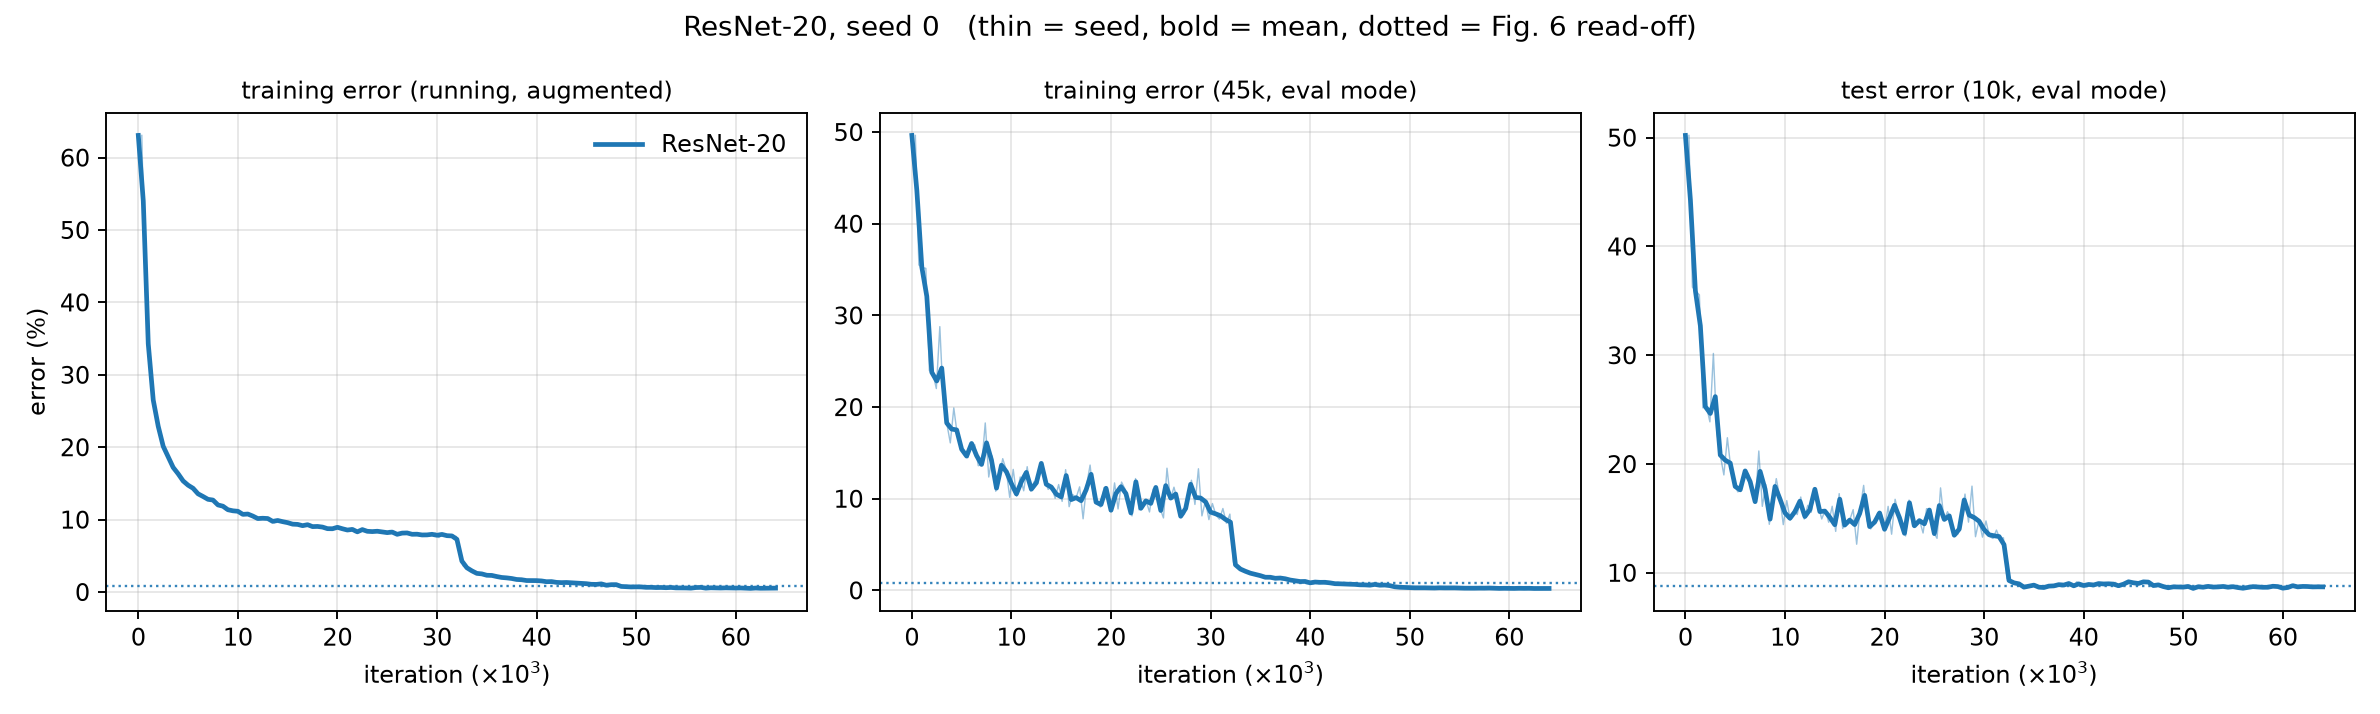
\includegraphics[width=\textwidth]{figures/milestone2.png}
\end{center}
\vspace{-6pt}
\begin{center}
\footnotesize{ResNet-20, seed~0. Left: running training error on the augmented
minibatches. Middle: training error on the 45{,}000 training images in
evaluation mode. Right: test error on the 10{,}000 test images. The dotted
lines are the values read off Figure~6 of the paper (0.8\% training, 8.8\%
test). The two drops are the learning-rate divisions at 32{,}000 and 48{,}000
iterations.}
\end{center}

\section{Errors after every epoch}

The table lists, after each of the 183 epochs, the running training error
(augmented, training mode), the training/validation/test errors (evaluation
mode, un-augmented), and the mean training loss over the epoch. The final row
is iteration 64{,}000, where the last epoch stops.

\begin{center}
\footnotesize
\begin{longtable}{@{}rrrrrrrr@{}}
\toprule
Epoch & Iter & lr & Training (running) & Training 45k & Val 5k & Test 10k & Loss \\
\midrule
\endfirsthead
\toprule
Epoch & Iter & lr & Training (running) & Training 45k & Val 5k & Test 10k & Loss \\
\midrule
\endhead
\bottomrule
\endfoot
1 & 351 & 0.1 & 63.07 & 49.64 & 49.30 & 50.21 & 0.0132 \\
2 & 702 & 0.1 & 41.73 & 35.50 & 34.92 & 36.26 & 0.0090 \\
3 & 1053 & 0.1 & 32.95 & 35.22 & 34.92 & 35.88 & 0.0072 \\
4 & 1404 & 0.1 & 27.45 & 35.14 & 35.50 & 35.55 & 0.0061 \\
5 & 1755 & 0.1 & 24.07 & 23.99 & 23.70 & 25.17 & 0.0054 \\
6 & 2106 & 0.1 & 22.39 & 23.71 & 23.64 & 25.33 & 0.0050 \\
7 & 2457 & 0.1 & 20.28 & 22.02 & 22.68 & 23.88 & 0.0046 \\
8 & 2808 & 0.1 & 19.15 & 28.78 & 29.08 & 30.17 & 0.0043 \\
9 & 3159 & 0.1 & 18.30 & 20.51 & 22.38 & 22.91 & 0.0041 \\
10 & 3510 & 0.1 & 17.18 & 18.20 & 19.78 & 20.77 & 0.0039 \\
11 & 3861 & 0.1 & 16.49 & 16.09 & 17.56 & 19.00 & 0.0037 \\
12 & 4212 & 0.1 & 16.11 & 19.91 & 21.32 & 22.42 & 0.0036 \\
13 & 4563 & 0.1 & 15.18 & 16.99 & 18.42 & 19.58 & 0.0034 \\
14 & 4914 & 0.1 & 14.83 & 15.52 & 17.02 & 18.10 & 0.0034 \\
15 & 5265 & 0.1 & 14.53 & 15.01 & 16.58 & 17.44 & 0.0033 \\
16 & 5616 & 0.1 & 14.24 & 14.48 & 16.78 & 17.72 & 0.0032 \\
17 & 5967 & 0.1 & 13.60 & 16.05 & 18.46 & 19.40 & 0.0031 \\
18 & 6318 & 0.1 & 13.31 & 15.89 & 18.02 & 19.09 & 0.0030 \\
19 & 6669 & 0.1 & 13.10 & 13.60 & 16.90 & 17.73 & 0.0029 \\
20 & 7020 & 0.1 & 12.79 & 13.75 & 16.02 & 16.47 & 0.0029 \\
21 & 7371 & 0.1 & 12.88 & 18.27 & 20.26 & 21.20 & 0.0028 \\
22 & 7722 & 0.1 & 12.41 & 12.37 & 15.62 & 16.11 & 0.0028 \\
23 & 8073 & 0.1 & 11.93 & 14.66 & 16.80 & 18.11 & 0.0027 \\
24 & 8424 & 0.1 & 12.01 & 10.82 & 13.88 & 14.46 & 0.0027 \\
25 & 8775 & 0.1 & 11.32 & 12.39 & 16.16 & 16.66 & 0.0026 \\
26 & 9126 & 0.1 & 11.39 & 14.37 & 17.86 & 18.66 & 0.0026 \\
27 & 9477 & 0.1 & 11.22 & 13.13 & 17.04 & 16.94 & 0.0026 \\
28 & 9828 & 0.1 & 11.26 & 10.15 & 13.50 & 14.43 & 0.0025 \\
29 & 10179 & 0.1 & 11.04 & 13.20 & 16.02 & 16.64 & 0.0025 \\
30 & 10530 & 0.1 & 10.70 & 10.27 & 13.88 & 14.86 & 0.0024 \\
31 & 10881 & 0.1 & 10.88 & 12.37 & 15.36 & 15.76 & 0.0024 \\
32 & 11232 & 0.1 & 10.57 & 10.87 & 14.12 & 15.36 & 0.0024 \\
33 & 11583 & 0.1 & 10.47 & 13.50 & 16.16 & 16.97 & 0.0024 \\
34 & 11934 & 0.1 & 10.16 & 10.85 & 14.70 & 14.94 & 0.0023 \\
35 & 12285 & 0.1 & 10.10 & 11.88 & 15.28 & 16.20 & 0.0023 \\
36 & 12636 & 0.1 & 10.25 & 11.65 & 14.60 & 15.57 & 0.0023 \\
37 & 12987 & 0.1 & 10.17 & 13.93 & 16.96 & 17.74 & 0.0023 \\
38 & 13338 & 0.1 & 9.93 & 12.05 & 15.32 & 16.21 & 0.0022 \\
39 & 13689 & 0.1 & 9.57 & 11.02 & 14.88 & 14.95 & 0.0022 \\
40 & 14040 & 0.1 & 9.92 & 11.31 & 14.86 & 15.77 & 0.0022 \\
41 & 14391 & 0.1 & 9.73 & 10.04 & 14.48 & 14.65 & 0.0022 \\
42 & 14742 & 0.1 & 9.71 & 11.55 & 15.04 & 16.12 & 0.0022 \\
43 & 15093 & 0.1 & 9.54 & 9.71 & 13.44 & 13.81 & 0.0021 \\
44 & 15444 & 0.1 & 9.36 & 13.17 & 17.18 & 17.28 & 0.0021 \\
45 & 15795 & 0.1 & 9.50 & 9.13 & 12.64 & 14.08 & 0.0021 \\
46 & 16146 & 0.1 & 9.23 & 10.46 & 14.78 & 14.61 & 0.0021 \\
47 & 16497 & 0.1 & 9.17 & 10.11 & 13.78 & 14.84 & 0.0020 \\
48 & 16848 & 0.1 & 9.22 & 11.30 & 15.26 & 15.81 & 0.0021 \\
49 & 17199 & 0.1 & 9.42 & 7.81 & 11.92 & 12.63 & 0.0021 \\
50 & 17550 & 0.1 & 8.98 & 11.50 & 15.34 & 15.92 & 0.0020 \\
51 & 17901 & 0.1 & 9.07 & 13.67 & 17.66 & 18.04 & 0.0020 \\
52 & 18252 & 0.1 & 9.04 & 10.10 & 13.88 & 14.78 & 0.0020 \\
53 & 18603 & 0.1 & 8.95 & 9.43 & 13.22 & 14.03 & 0.0020 \\
54 & 18954 & 0.1 & 8.74 & 9.09 & 13.04 & 14.53 & 0.0019 \\
55 & 19305 & 0.1 & 8.87 & 11.22 & 14.66 & 15.52 & 0.0020 \\
56 & 19656 & 0.1 & 8.64 & 11.08 & 15.20 & 15.49 & 0.0019 \\
57 & 20007 & 0.1 & 8.95 & 8.70 & 12.84 & 13.97 & 0.0020 \\
58 & 20358 & 0.1 & 8.78 & 11.73 & 15.88 & 16.11 & 0.0019 \\
59 & 20709 & 0.1 & 8.69 & 8.89 & 12.92 & 13.55 & 0.0019 \\
60 & 21060 & 0.1 & 8.54 & 11.82 & 16.40 & 16.76 & 0.0019 \\
61 & 21411 & 0.1 & 8.80 & 11.05 & 14.08 & 15.38 & 0.0019 \\
62 & 21762 & 0.1 & 8.22 & 9.13 & 13.22 & 14.15 & 0.0018 \\
63 & 22113 & 0.1 & 8.36 & 8.13 & 12.56 & 13.39 & 0.0019 \\
64 & 22464 & 0.1 & 8.64 & 12.20 & 16.34 & 16.69 & 0.0019 \\
65 & 22815 & 0.1 & 8.54 & 8.79 & 12.98 & 14.27 & 0.0019 \\
66 & 23166 & 0.1 & 8.26 & 9.10 & 13.14 & 14.37 & 0.0018 \\
67 & 23517 & 0.1 & 8.36 & 9.80 & 13.90 & 14.82 & 0.0019 \\
68 & 23868 & 0.1 & 8.43 & 8.56 & 12.88 & 13.66 & 0.0019 \\
69 & 24219 & 0.1 & 8.35 & 11.04 & 15.84 & 15.90 & 0.0018 \\
70 & 24570 & 0.1 & 8.30 & 11.28 & 15.52 & 15.74 & 0.0018 \\
71 & 24921 & 0.1 & 8.12 & 8.96 & 13.32 & 13.73 & 0.0018 \\
72 & 25272 & 0.1 & 8.51 & 7.91 & 11.70 & 13.17 & 0.0019 \\
73 & 25623 & 0.1 & 8.16 & 13.33 & 17.26 & 17.81 & 0.0018 \\
74 & 25974 & 0.1 & 7.96 & 9.97 & 13.84 & 14.85 & 0.0018 \\
75 & 26325 & 0.1 & 8.14 & 11.26 & 14.96 & 15.62 & 0.0018 \\
76 & 26676 & 0.1 & 8.14 & 9.77 & 15.42 & 14.85 & 0.0018 \\
77 & 27027 & 0.1 & 8.17 & 7.95 & 12.56 & 13.34 & 0.0018 \\
78 & 27378 & 0.1 & 7.94 & 8.33 & 13.38 & 13.57 & 0.0017 \\
79 & 27729 & 0.1 & 8.04 & 10.08 & 14.44 & 14.86 & 0.0018 \\
80 & 28080 & 0.1 & 7.97 & 12.02 & 16.44 & 17.24 & 0.0018 \\
81 & 28431 & 0.1 & 7.86 & 9.38 & 13.84 & 14.66 & 0.0017 \\
82 & 28782 & 0.1 & 7.97 & 13.27 & 18.00 & 17.97 & 0.0018 \\
83 & 29133 & 0.1 & 7.85 & 8.13 & 12.84 & 13.32 & 0.0017 \\
84 & 29484 & 0.1 & 7.97 & 9.75 & 14.12 & 14.81 & 0.0017 \\
85 & 29835 & 0.1 & 8.13 & 7.72 & 12.26 & 13.28 & 0.0018 \\
86 & 30186 & 0.1 & 7.53 & 9.48 & 13.34 & 14.77 & 0.0017 \\
87 & 30537 & 0.1 & 8.01 & 8.23 & 12.96 & 13.35 & 0.0018 \\
88 & 30888 & 0.1 & 7.73 & 7.77 & 12.46 & 13.16 & 0.0017 \\
89 & 31239 & 0.1 & 7.92 & 8.93 & 13.24 & 13.93 & 0.0018 \\
90 & 31590 & 0.1 & 7.69 & 7.33 & 12.36 & 13.13 & 0.0017 \\
91 & 31941 & 0.1 & 7.68 & 8.32 & 12.98 & 13.22 & 0.0017 \\
92 & 32292 & 0.01 & 5.31 & 3.08 & 8.56 & 9.48 & 0.0012 \\
93 & 32643 & 0.01 & 3.57 & 2.59 & 8.26 & 9.17 & 0.0008 \\
94 & 32994 & 0.01 & 3.36 & 2.33 & 8.24 & 9.08 & 0.0008 \\
95 & 33345 & 0.01 & 3.01 & 2.16 & 8.44 & 9.01 & 0.0007 \\
96 & 33696 & 0.01 & 2.83 & 2.00 & 8.00 & 8.96 & 0.0007 \\
97 & 34047 & 0.01 & 2.54 & 1.86 & 8.08 & 8.64 & 0.0006 \\
98 & 34398 & 0.01 & 2.59 & 1.75 & 8.20 & 8.77 & 0.0006 \\
99 & 34749 & 0.01 & 2.31 & 1.74 & 8.22 & 8.79 & 0.0006 \\
100 & 35100 & 0.01 & 2.32 & 1.56 & 8.06 & 8.90 & 0.0005 \\
101 & 35451 & 0.01 & 2.33 & 1.42 & 8.10 & 8.69 & 0.0005 \\
102 & 35802 & 0.01 & 2.12 & 1.52 & 8.12 & 8.62 & 0.0005 \\
103 & 36153 & 0.01 & 2.16 & 1.37 & 8.26 & 8.67 & 0.0005 \\
104 & 36504 & 0.01 & 2.01 & 1.32 & 8.02 & 8.78 & 0.0005 \\
105 & 36855 & 0.01 & 2.02 & 1.44 & 7.92 & 8.71 & 0.0005 \\
106 & 37206 & 0.01 & 1.87 & 1.23 & 8.22 & 8.93 & 0.0004 \\
107 & 37557 & 0.01 & 1.87 & 1.28 & 8.38 & 8.91 & 0.0004 \\
108 & 37908 & 0.01 & 1.75 & 1.16 & 8.04 & 8.86 & 0.0004 \\
109 & 38259 & 0.01 & 1.70 & 1.04 & 8.16 & 8.92 & 0.0004 \\
110 & 38610 & 0.01 & 1.70 & 1.06 & 8.04 & 9.06 & 0.0004 \\
111 & 38961 & 0.01 & 1.59 & 0.96 & 7.96 & 8.76 & 0.0004 \\
112 & 39312 & 0.01 & 1.59 & 1.03 & 8.34 & 9.18 & 0.0004 \\
113 & 39663 & 0.01 & 1.59 & 0.93 & 7.92 & 8.81 & 0.0004 \\
114 & 40014 & 0.01 & 1.58 & 0.82 & 8.14 & 8.83 & 0.0004 \\
115 & 40365 & 0.01 & 1.56 & 0.92 & 8.30 & 8.95 & 0.0004 \\
116 & 40716 & 0.01 & 1.50 & 0.90 & 8.32 & 8.90 & 0.0004 \\
117 & 41067 & 0.01 & 1.41 & 0.87 & 8.16 & 8.88 & 0.0003 \\
118 & 41418 & 0.01 & 1.46 & 0.89 & 8.56 & 9.02 & 0.0003 \\
119 & 41769 & 0.01 & 1.39 & 0.86 & 8.12 & 8.99 & 0.0003 \\
120 & 42120 & 0.01 & 1.31 & 0.80 & 8.04 & 8.97 & 0.0003 \\
121 & 42471 & 0.01 & 1.30 & 0.74 & 8.00 & 9.01 & 0.0003 \\
122 & 42822 & 0.01 & 1.28 & 0.68 & 8.64 & 8.80 & 0.0003 \\
123 & 43173 & 0.01 & 1.36 & 0.76 & 8.28 & 9.12 & 0.0003 \\
124 & 43524 & 0.01 & 1.28 & 0.69 & 8.14 & 8.79 & 0.0003 \\
125 & 43875 & 0.01 & 1.27 & 0.66 & 8.28 & 8.90 & 0.0003 \\
126 & 44226 & 0.01 & 1.18 & 0.70 & 8.40 & 9.06 & 0.0003 \\
127 & 44577 & 0.01 & 1.19 & 0.64 & 8.12 & 9.21 & 0.0003 \\
128 & 44928 & 0.01 & 1.16 & 0.59 & 8.32 & 9.10 & 0.0003 \\
129 & 45279 & 0.01 & 1.16 & 0.70 & 8.34 & 9.01 & 0.0003 \\
130 & 45630 & 0.01 & 1.02 & 0.54 & 7.96 & 9.03 & 0.0003 \\
131 & 45981 & 0.01 & 1.05 & 0.57 & 8.02 & 9.17 & 0.0003 \\
132 & 46332 & 0.01 & 1.08 & 0.57 & 8.24 & 9.19 & 0.0003 \\
133 & 46683 & 0.01 & 1.18 & 0.74 & 8.84 & 9.10 & 0.0003 \\
134 & 47034 & 0.01 & 0.92 & 0.55 & 8.32 & 8.80 & 0.0002 \\
135 & 47385 & 0.01 & 0.99 & 0.55 & 8.20 & 8.90 & 0.0002 \\
136 & 47736 & 0.01 & 1.07 & 0.66 & 8.60 & 8.88 & 0.0003 \\
137 & 48087 & 0.001 & 1.01 & 0.48 & 8.38 & 8.69 & 0.0002 \\
138 & 48438 & 0.001 & 0.79 & 0.40 & 8.30 & 8.61 & 0.0002 \\
139 & 48789 & 0.001 & 0.72 & 0.38 & 8.36 & 8.71 & 0.0002 \\
140 & 49140 & 0.001 & 0.75 & 0.32 & 8.18 & 8.71 & 0.0002 \\
141 & 49491 & 0.001 & 0.71 & 0.33 & 8.16 & 8.70 & 0.0002 \\
142 & 49842 & 0.001 & 0.68 & 0.32 & 7.96 & 8.66 & 0.0002 \\
143 & 50193 & 0.001 & 0.77 & 0.29 & 8.16 & 8.72 & 0.0002 \\
144 & 50544 & 0.001 & 0.70 & 0.28 & 8.20 & 8.75 & 0.0002 \\
145 & 50895 & 0.001 & 0.62 & 0.28 & 8.10 & 8.56 & 0.0002 \\
146 & 51246 & 0.001 & 0.73 & 0.29 & 8.12 & 8.59 & 0.0002 \\
147 & 51597 & 0.001 & 0.63 & 0.28 & 8.18 & 8.77 & 0.0002 \\
148 & 51948 & 0.001 & 0.61 & 0.28 & 8.08 & 8.67 & 0.0002 \\
149 & 52299 & 0.001 & 0.66 & 0.25 & 8.02 & 8.72 & 0.0002 \\
150 & 52650 & 0.001 & 0.61 & 0.27 & 8.12 & 8.78 & 0.0002 \\
151 & 53001 & 0.001 & 0.60 & 0.28 & 8.00 & 8.69 & 0.0002 \\
152 & 53352 & 0.001 & 0.63 & 0.26 & 8.16 & 8.69 & 0.0002 \\
153 & 53703 & 0.001 & 0.64 & 0.28 & 8.18 & 8.73 & 0.0002 \\
154 & 54054 & 0.001 & 0.57 & 0.27 & 8.16 & 8.75 & 0.0002 \\
155 & 54405 & 0.001 & 0.58 & 0.28 & 7.98 & 8.67 & 0.0002 \\
156 & 54756 & 0.001 & 0.55 & 0.26 & 8.14 & 8.70 & 0.0002 \\
157 & 55107 & 0.001 & 0.57 & 0.25 & 8.22 & 8.74 & 0.0002 \\
158 & 55458 & 0.001 & 0.53 & 0.24 & 8.26 & 8.65 & 0.0002 \\
159 & 55809 & 0.001 & 0.60 & 0.24 & 8.28 & 8.60 & 0.0002 \\
160 & 56160 & 0.001 & 0.64 & 0.23 & 7.92 & 8.57 & 0.0002 \\
161 & 56511 & 0.001 & 0.64 & 0.24 & 8.10 & 8.66 & 0.0002 \\
162 & 56862 & 0.001 & 0.53 & 0.26 & 8.24 & 8.72 & 0.0002 \\
163 & 57213 & 0.001 & 0.56 & 0.24 & 8.00 & 8.75 & 0.0002 \\
164 & 57564 & 0.001 & 0.59 & 0.25 & 8.10 & 8.69 & 0.0002 \\
165 & 57915 & 0.001 & 0.56 & 0.27 & 8.10 & 8.66 & 0.0002 \\
166 & 58266 & 0.001 & 0.61 & 0.24 & 8.18 & 8.70 & 0.0002 \\
167 & 58617 & 0.001 & 0.53 & 0.24 & 8.02 & 8.66 & 0.0002 \\
168 & 58968 & 0.001 & 0.58 & 0.22 & 8.02 & 8.77 & 0.0002 \\
169 & 59319 & 0.001 & 0.55 & 0.22 & 8.00 & 8.72 & 0.0002 \\
170 & 59670 & 0.001 & 0.58 & 0.24 & 8.04 & 8.75 & 0.0002 \\
171 & 60021 & 0.001 & 0.55 & 0.22 & 7.92 & 8.58 & 0.0002 \\
172 & 60372 & 0.001 & 0.56 & 0.21 & 8.02 & 8.60 & 0.0002 \\
173 & 60723 & 0.001 & 0.58 & 0.22 & 7.92 & 8.74 & 0.0002 \\
174 & 61074 & 0.001 & 0.53 & 0.24 & 7.98 & 8.84 & 0.0002 \\
175 & 61425 & 0.001 & 0.49 & 0.22 & 7.90 & 8.71 & 0.0001 \\
176 & 61776 & 0.001 & 0.56 & 0.23 & 7.92 & 8.70 & 0.0002 \\
177 & 62127 & 0.001 & 0.55 & 0.23 & 7.96 & 8.78 & 0.0002 \\
178 & 62478 & 0.001 & 0.52 & 0.21 & 8.18 & 8.74 & 0.0002 \\
179 & 62829 & 0.001 & 0.55 & 0.21 & 8.04 & 8.75 & 0.0002 \\
180 & 63180 & 0.001 & 0.51 & 0.22 & 8.16 & 8.66 & 0.0001 \\
181 & 63531 & 0.001 & 0.54 & 0.21 & 7.94 & 8.72 & 0.0001 \\
182 & 63882 & 0.001 & 0.56 & 0.21 & 8.04 & 8.79 & 0.0002 \\
183 & 64000 & 0.001 & 0.54 & 0.22 & 7.96 & 8.71 & 0.0002 \\
\end{longtable}
\end{center}

\section{Wall-clock time}

The run took 17.6\ minutes of wall-clock time on one RTX 4060 Laptop GPU,
that is 16.5\ milliseconds per training iteration including the four error
measurements taken every 351 iterations. For the full replication this sets the
budget: the 20-layer networks cost about 16 minutes and the 56-layer networks
about 50 minutes per run, so the twelve runs of the main experiment need
roughly five hours of GPU time on this machine.

\section{Deviations from the paper}

\begin{itemize}
\item \textbf{45{,}000 training images.} The card fixes the split; the paper
does not say whether the networks behind Table~6 saw 45{,}000 or 50{,}000
images. Fewer training images can only make our errors higher than the
paper's, and our 8.71\% is not higher, so the split is not inflating the gap.
\item \textbf{Batch 128 on one GPU.} The paper trains with batch 128 ``on two
GPUs'' (Sec.~4.2); the card fixes the batch at 128, so we keep the same
effective batch on a single device.
\item \textbf{Mixed precision.} The card permits float16 autocast with gradient
scaling provided it is used in \emph{every} run; every run reported here and in
the final report uses it, and all reported errors are measured in float32.
\end{itemize}

\section*{AI use declaration}
We used Claude Code (Anthropic) as a coding assistant: it wrote the training
and evaluation code, the table and figure scripts, and drafted this milestone.
The recipe and protocol were taken from the paper and the topic card by the
team; every number in this document is generated by the scripts from the run's
own output files, and all code and experiments are run and understood by the
team, and every member can explain every line and every plot, as the course
requires.

\end{document}
